% mainfile: ../../../../master.tex
\subsection{SELinux Syntax}
\label{task:20231219_selinux}

SELinux Tutorials from \footnote{\url{https://wiki.gentoo.org/wiki/SELinux/Tutorials}}.

\subsubsection{The security context of a process}

The security context, together with the run-time user that the process is in, would define what the process is allowed to do.

\begin{lstlisting}[language=sh]
ps -ef # -e gives all processes, -f gives more info, -Z gives security context

ls -ld dir # shows the permissions related to this directory
ls -ldZ dir # shows the permissions and also SELinux context
\end{lstlisting}

\begin{itemize}
\item \textbf{Domain.} The context of the process that is acting upon something.
\item \textbf{Type.} The context of the resource on which the process is acting.
\item \textbf{Class.} The object class of the resource (e.g. \textit{file} or \textit{socket}).
\item \textbf{Permissions.} The permissions that are allowed given the \textit{domain}, \textit{type} and \textit{class}.
\end{itemize}

SELinux rule syntax:
\begin{lstlisting}
allow <domain> <type>:<class> { <permissions> };
\end{lstlisting}

\subsubsection{Decoding Permission Denial Message}

Message:
\begin{lstlisting}
type=AVC msg=audit(1363289005.532:184): avc:  denied  { read } for  pid=29199 comm="Trace" 
name="online" dev="sysfs" ino=30 scontext=staff_u:staff_r:googletalk_plugin_t 
tcontext=system_u:object_r:sysfs_t tclass=file
\end{lstlisting}

\begin{longtable}{p{.15\linewidth}p{.15\linewidth}p{.65\linewidth}} 
\toprule
Log part & Name & Description \\
\midrule
\endhead

\texttt{type=AVC}
&Log type
&Only in the \texttt{audit.log} file; it informs the user what kind of audit log type this is. 
\\

\texttt{msg=audit(1363289005.532:184)}
&Timestamp
&Timestamp in seconds since epoch, meaning the number of seconds since January 1st, 1970. You can convert this to a more human readable format using date -d @ followed by the number, like so: \texttt{date -d @1363292159.532}.
\\

\texttt{avc:}
&Log type (again)
&
\\

\texttt{denied}
&State (if enforced)
&What SELinux did, which can be either \texttt{denied} or \texttt{granted}. Note that, if SELinux is in premissive mode, then it will still log as \texttt{denied} even though it was enforced.
\\

\texttt{\{ read \}}
&Permission
&Ther permission that was requested or executed. In this case, it is a read operation. Sometimes the permission contains a set like \texttt{\{ read write \}} but in most cases, it is a single permission request.
\\

\texttt{for pid=29199}
&Process PID
&Ther process identifier of the process that took the action.
\\

\texttt{comm="Trace"}
&Process CMD
&The process command (without arguments, and limited to 15 characters), which helps users identify what the process was in case the process is already gone (a PID is only useful if the process is still running)
\\

\texttt{name="online"}
&Target name
&The name of the target (in this case, file name). This field depends heavily on the target itself; it can also be \texttt{path=}, \texttt{capability=}, \texttt{src=} and more. But in those cases, its purposes should be clear from the rest of the log.
\\

\texttt{dev="sysfs"}
&Device
&Device on which the target (in case of a file or file system). In this case, the device is \texttt{sysfs} so we have the hint immediately that this is for something inside \texttt{/sys}. Other valid example are \texttt{dev=md-0}, \texttt{dev=sda1}, or \texttt{dev=tmpfs}.
\\

\texttt{ino=30}
&inode number
&The inode number of the target file. In this case, since we know it is on the \texttt{sysfs} file system, we can look for this file using: \texttt{find /sys -xdev -inum 30}
\\

\texttt{scontent=staff\_u:staff\_r:googletalk\_plugin\_t}
&Source context
&The security context of the process (the domain)
\\

\texttt{tcontext=system\_u:object\_r:sysfs\_t}
&Target context
&The security context of the target resource (in this case the file)
\\

\texttt{tclass=file}
&Target class
&The class of the target.
\\

\midrule
\caption{Permission Denied Syntax} 
\label{tab:permissiondeniedsyntax}
\end{longtable}


% \subsubsection{SELinux Architecture}

% SELinux consists of four main components: object managers (OM), access vector cache (AVC), security server, and security policy as show below:
% \begin{figure}[H]
%     \centering
%     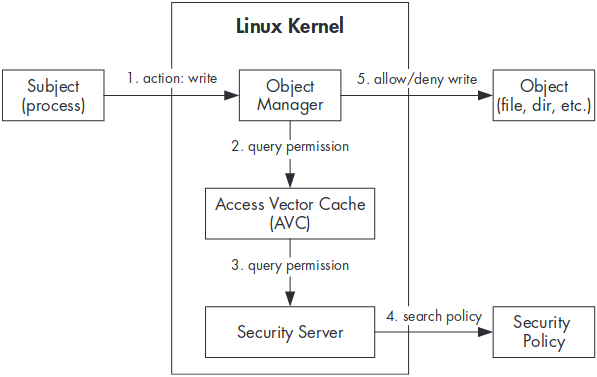
\includegraphics[width=.85\linewidth]{entries/2023/12/10/selinux.png}
%     \caption{SELinux Components}
%     \label{fig:selinux}
% \end{figure}
% When a subject asks to perform an action on an SELinux object, the associated object manager queries the AVC to see if the attempted action is allowed. If the AVC contains a cached security decision for the request, the AVC returns it to the OM which enforces the decision by allowing or denying the action. If the cache does not contain a matching security decision based on the currently loaded policy and returns it to the AVC, which caches it. The AVC in turn returns it to the OM which ultimately enforces the decision. The security server is part of the kernel, while the policy is loaded from userspace via a series of functions contained in the supporting userspace library.

% \subsubsection{SELinux Modes}

% SELinux has 3 modes:
% \begin{itemize}
% \item \textbf{Disabled.} No policy is loaded and only the default DAC security is enforced.
% \item \textbf{Permissive.} The policy is loaded and object access is checked, but access denial is only logged - not enforced.
% \item \textbf{Enforcing.} The security policy is both loaded and enforced, with violations logged.
% \end{itemize}

% SELinux mode can be checked and changed with the \texttt{getenforce} and \texttt{setenforce} commands:
% \begin{lstlisting}[language=sh]
% # getenforce
% Enforcing
% # setenforce 0
% # getenforce
% Permissive
% \end{lstlisting}
% The mode set with \texttt{setenforce} is not persistent and will be reset to the default mode when the device reboots.

% \subsubsection{Mandatory Access Control}

% \begin{itemize}
% \item \textbf{Subjects} are usually running processes that perform actions on objects,
% \item \textbf{Objects} are OS-level resources managed by the kernel (processes can also be objects), and
% \item \textbf{Actions} are carried out only if the security policy allows it.
% \end{itemize}
% Both subjects and objects have a set of security attributes (collectively known as the security context) which the OS queries in order to decide whether the requested action should be allowed or not. When SELinux is enabled, subjects cannot bypass or influence policy rules; therefore, the policy is mandatory. The MAC policy is only consulted if the DAC allows access to the resource. If the DAC denies access, the denial is taken as the final security decision. 

% % \noindent
% SELinux support two forms of MAC: \textit{type enforcement (TE)} and \textit{multi-level security (MLS)}. 
% MLS is used to enforce different levels of access to restricted information and is not used in Android. 
% TE implemented in SELinux requires that all subjects and objects have an associated type and SELinux uses this type to enforce the rules of its security policy. A \textit{type} is simply a string that's defined in the policy and assoicated with objects or subjects. Subject types references processes or groups of processes and are also referred to as \textit{domains}. Types referring to objects usually specify the role an object plays within a policy, such as system file, application data file, and so on. The type (or domain) is an integral part of the security context.

% \subsubsection{Security Contexts}

% A \textit{security context} (also referred to as a \textit{security label}, or just \textit{label}) is a string with four fields delimited with colons: username, role, type, and an optional MLS security range. 

% An SELinux username is typically asosciated with a group of class of users; for example \path{user_u} for unprivileged users and \path{admin_u} for administrators. Users can be associated with one or more domain type. The type is used to group processes in a domain or to specify an object logical type. In Android context, the user is fixed to \texttt{u}.

% The security range (or level) is used to implement ML and specifies the security levels a subject is allowed to access. In Android context, the security range is fixed to \texttt{s0}.

% By specifying the option \texttt{-Z}, we can see the security context of the processes running:
% \begin{lstlisting}[language=sh]
% # ps -Z
% u:r:su:s0   root    1847    1834    10842820    3384    sigsuspe+
% u:r:su:s0   root    1878    1847    10800932    3572    0  
% \end{lstlisting}
% Subjects inherit the security context of their parent process, or they can change their context via \textit{domain transition} which can be made automatic. For example, all system daemons are started by the \textit{init} process, which has \textit{u:r:init:s0} secuirty context, they would normally inherit this context, but Android's SELinux poly uses automatic domain transitions to set a dedicated domain to each daemon as need.

% Similarly the context of files can be revealed using the \texttt{-Z} option:
% \begin{lstlisting}[language=sh]
% # ls -Z
% lrwxr-xr-x 1 root shell u:object_r:system_file:s0                         6 2023-11-19 00:50 uuidgen -> toybox
% -rwxr-xr-x 1 root shell u:object_r:vdc_exec:s0                       101920 2023-11-19 00:50 vdc
% -rwxr-xr-x 1 root shell u:object_r:viewcompiler_exec:s0              277472 2023-11-19 00:50 viewcompiler
% lrwxr-xr-x 1 root shell u:object_r:system_file:s0                         6 2023-11-19 00:50 vmstat -> toybox
% -rwxr-xr-x 1 root shell u:object_r:vold_exec:s0                      994368 2023-11-19 00:50 vold
% -rwxr-xr-x 1 root shell u:object_r:vold_prepare_subdirs_exec:s0       38576 2023-11-19 00:50 vold_prepare_subdirs
% -rwxr-xr-x 1 root shell u:object_r:system_file:s0                       169 2023-11-19 01:02 vr
% lrwxr-xr-x 1 root shell u:object_r:system_file:s0                         6 2023-11-19 00:50 watch -> toybox
% -rwxr-xr-x 1 root shell u:object_r:watchdogd_exec:s0                  10760 2023-11-19 00:50 watchdogd
% lrwxr-xr-x 1 root shell u:object_r:system_file:s0                         6 2023-11-19 00:50 wc -> toybox
% lrwxr-xr-x 1 root shell u:object_r:system_file:s0                         6 2023-11-19 00:50 which -> toybox
% lrwxr-xr-x 1 root shell u:object_r:system_file:s0                         6 2023-11-19 00:50 whoami -> toybox
% -rwxr-xr-x 1 root shell u:object_r:wificond_exec:s0                  393248 2023-11-19 00:50 wificond

% \end{lstlisting}
% For objects, the security context is persistent and is usually stored as an extended attribute in the file's metadata. Objects typically inherit the type label of their parent (their directory), and can change to a different label via \textit{type transition}.

% \subsubsection{Security Policy}

% Security policies are used by the security server in the kernel to allow or disallow access to kernel objects at runtime. For performance reasons, the policy is typically in binary form generated by compiling a number of policy source files. \textit{Statements} define policy entities such as types, users, and roles. \textit{Rules} allow or deny access to objects (access vector rules); and designate how default users, roles, and types are assigned (default rules). \footnote{Type, attribute and permission statements make up the bulk of a security policy.}

% The listing below declares \path{file_type} and \texttt{domain} attributes, declares \path{system_data_file} type and associates it with \path{file_type} and \path{data_file_type} attributes, declares \path{untrusted_app} type and associate it with \texttt{domain} attribute:
% \begin{lstlisting}
% attribute file_type;
% attribute domain;

% type system_data_file, file_type, data_file_type;
% type untrusted_app, domain;
% \end{lstlisting}

% \texttt{user} statement declares an SELinux user identifier, associates it with its role(s), and optionally specifies its default security level and the range of security levels that user can access:
% \begin{lstlisting}
% user u roles { r } level s0 range s0 - mls_systemhigh;
% \end{lstlisting}
% The \textit{u} user is associated with the \textit{r} role (inside the braces), which in turn is declared using the \texttt{role} statement as show below:
% \begin{lstlisting}
% role r;
% role r types domain;
% \end{lstlisting}
% The second statement associates the \textit{r} role with the \texttt{domain} attribute, which marks it as a role assigned to processes (domains).

% \texttt{permissive} statement allows a named domain to run in permissive mode\footnote{Most domains in Android's current base policy are permissive.}:
% \begin{lstlisting}
% type adbd, domain;
% permissive adbd;
% --snip--
% \end{lstlisting}

% The \texttt{class} statement defines an SELinux object class. Object classes and their associated permissions are determined by the respected object manager implementations in Linux kernel, and are static within a policy. Object classes are usually defined in the \textit{security\_classes} policy source file:
% \begin{lstlisting}
% --snip-
% # file-related classes 
% class filesystem 
% class file 
% class dir 
% class fd 
% class lnk_file 
% class chr_file 
% class blk_file 
% class sock_file 
% class fifo_file 
% --snip--
% \end{lstlisting}

% Access vectors are usually defined and associated with object classes in a policy source file called \textit{access\_vectors}. Permissions can be either class-specific or inheritable by one or more object classes, in which case they're defined with the \texttt{common} keyword. Below is the definition of the set of permissions common to all file objects, and the association of the \texttt{dir} class (which represents directories), and a set of directory-specific permissions (\textit{add\_name}, \textit{remove\_name}, and so on):
% \begin{lstlisting}
% --snip--
% common file 
% { 
%     ioctl 
%     read
%     write 
%     create 
%     getattr 
%     setattr 
%     lock 
%     --snip--
% } 
% --snip--
% class dir 
% inherits file 
% { 
%     add_name 
%     remove_name 
%     reparent 
%     search 
%     rmdir 
%     --snip--
% }
% --snip--
% \end{lstlisting}

% \subsubsection{Type Transition Rules}

% Type enforcement rules and access vector rules typically make the bulk of an SELinux policy. The most commonly used type of enforcement rule is the \path{type_transition} rule, which specifies when domain and type transitions are allowed:
% \begin{lstlisting}
% # from wpa_supplicant.te

% # wpa - wpa supplicant or equivalent 
% type wpa, domain; 
% permissive wpa;
% type wpa_exec, exec_type, file_type; 

% init_daemon_domain(wpa)
% unconfined_domain(wpa)

% # wpa_supplicant daemon uses the type transition rule to associate the control sockets it creates in /data/misc/wifi directory with wpa_socket type
% type_transition wpa             wifi_data_file: sock_file   wpa_socket;
% #               source type     target type     class       type of object after the transition
% \end{lstlisting}

% \subsubsection{Domain Transition Rules}

% Most daemons are associated with a dedicated and use domain transitions to switch their domain when started. This is typically accomplished using the \path{init_daemon_domain()} macro, which under the hood is implemented using the \path{type_transition} keyword. The \path{init_daemon_domain()} macro takes one parameter and is defined in the \textit{te\_macros} file using two other macros: \path{domain_trans()} and \path{domain_auto_trans()} which are used to allow transition to a new domain and to execute the transition automatically, respectively:
% \begin{lstlisting}
% # Domain transition macros definition int the te_macros file

% # domain_trans(olddomain, type, newdomain) 
% define(`domain_trans', ` 
% allow $1 $2:file { getattr open read execute }; 
% allow $1 $3:process transition; 
% allow $3 $2:file { entrypoint read execute }; 
% allow $3 $1:process sigchld; 
% dontaudit $1 $3:process noatsecure; 
% allow $1 $3:process { siginh rlimitinh }; ')
% # domain_auto_trans(olddomain, type, newdomain) 
% define(`domain_auto_trans', ` 
% domain_trans($1,$2,$3) 
% type_transition $1 $2:process $3; ')
% # init_daemon_domain(domain) 
% define(`init_daemon_domain', ` 
% domain_auto_trans(init, $1_exec, $1) 
% tmpfs_domain($1) ') 
% --snip--
% \end{lstlisting}
% The lines beginning with the \texttt{allow} keyword are access vector (AV) rules.

% \subsubsection{Access Vector Rules}

% AV rules define what privileges processes have at runtime by specifying the set of permissions they have over their target objects:
% \begin{lstlisting}
% # Format of AV rules
% rule_name source_type target_type : class perm_set;
% \end{lstlisting}

% The \path{rule_name} can be \texttt{allow}, \texttt{dontallow}, \texttt{auditallow}, \texttt{neverallow}. 
% \texttt{allow} specifies the operations that a subject (process) of the specified source type is allowed to perform on an object of the target type and class specified in the rule.
% \texttt{auditallow} rule is used with \texttt{allow} to record audit events when an operation is allowed.
% \texttt{dontaudit} rule is used to suppress the auditing of denial messages when a specified event is known to be safe.
% \texttt{neverallow} rule says that the declared operation should never be allowed even if an explicit \texttt{allow} rule that allows it exists.

% To form a rule, \path{source_type} and \path{target_type} elements are replaced with one or more previously defined \texttt{type} or \texttt{attribute} identifiers, where \path{source_type} is the identifier of a subject (process), and \path{target_type} is the identifer of an object the process is trying to access. The \texttt{class} element is replaced with the object class of the target, and \path{perm_set} specifies the set of permissions that the source process has over the target object. You can specify multiple types, classes, and permissions by enclosing them in braces (\path{{}}). In addition, so rules support use of the wildcard (\path{*}) and complement(\path{~}) operators, which allow you to specify that all types should be included or that all types except those explicityly listed should be included, respectively:
% \begin{lstlisting}
% type vold, domain;
% type vold_exec, exec_type, file_type;
% init_daemon_domain(vold)

% # allows daemons running in vold domain to mount, unmount, and remount filesystems of sdcard_type
% allow vold sdcard_type:filesystem { mount remount unmount };

% # allows daemons running in vold domain to use the CAP_SYS_PTRACE and CAP_KILL Linux capabilities
% # self means that target domain is same as source (vold in this case)
% allow vold self:capability { sys_ptrace kill };

% type installd, domain;

% # no audit log will be created if the installd daemon is denied the CAP_SYS_ADMIN capability
% dontaudit installd self:capability sys_admin;

% # forbids all domains but the init domain to load the SELinux policy
% neverallow { domain -init } kernel:security load_policy;
% \end{lstlisting}